\documentclass[12pt,letterpaper]{article}
\usepackage[left=1in,top=1in,right=1in,bottom=1in,nohead]{geometry}
\pagestyle{empty}
\linespread{1.5}
\usepackage[T1]{fontenc}
\usepackage{ragged2e}
\usepackage{setspace}
\usepackage{mdwlist}
% \usepackage{array}
% \usepackage{multirow}
\usepackage{graphicx}
% \usepackage{wrapfig}
% \usepackage{longtable}
% \usepackage{subfig}
\usepackage{amsmath}
\usepackage{amssymb}
\usepackage{bbm}
\usepackage{dsfont}
\usepackage{mathptmx}
\usepackage[hang]{caption}
\DeclareMathAlphabet{\mathcal}{OMS}{cmsy}{m}{n}
\usepackage{relsize}
\usepackage{fancyvrb}
\def \fullline {\vspace{.2em}\hrule\vspace{3px}}

\begin{document}
\setlength{\parindent}{0.25in}
\setlength{\floatsep}{0in}
\section{Radial Density Function}
\subsection{Calculation of Distances with Periodicity}
Suppose a large chemical structure has uncountably many atoms but the follow a
periodic pattern of $n$ atoms every $p$ Angstroms. The atom locations within a
period are given by $a_1, a_2, \ldots, a_n$ where $a_i \in \mathbb{R}^3$. The
radial density function is the distribution of pairwise distances between these
atoms.

The distances $d$ between atoms $a_i$ and $a_j$ where $i \neq j$, atom $a_i$
has been displaced by $x$, and atom $a_j$ has been displaced by $y$ per the
periodicity is 
\begin{align*}
  d^2 &= \langle a_i + x - (a_j + y), a_i + x - (a_j + y) \rangle \\
      &= \langle a_i-a_j, a_i-a_j \rangle  + \langle x-y, x-y \rangle  
      + 2 \langle a_i-a_j,x-y \rangle 
\end{align*}
where $x =(k_1 p, k_2 p, k_3 p)$ for $k_i \in \mathbb{Z}$ 
and $y = (l_1 p, l_2 p, l_3 p)$ for $l_i \in \mathbb{Z}$.
Here $\langle x,y \rangle $ denotes the inner product between $x$ and $y$. 

Suppose $D$ is a random variable that samples at random the distances, $d$, in
the chemical structure. The radial density function is the probability density
function of this random variable. This function can be estimated empirically via
a histogram.

\subsection{Adding Noise For Atom Vibration}
Due to the vibrations of the molecules, the radial density function will not be
just the equilibrium positions. We can approximate this fluctuation in distances
via a Gaussian filter or Weierstrass transform.

\begin{align*}
F(x)=\frac{1}{\sqrt{4\pi t}} 
  \int_{-\infty}^\infty f(y) e^{-\frac{(x-y)^2}{4t}} dy
\end{align*}

Given that the density function is only defined for a finite number of
distances, we use a discrete version of the transform making sure to keep the
sum of the weights equal to one.

\begin{align*}
  F(d_k) = \frac{\sum_{d_i = d_0}^{d_n} f(d_i) \exp\left(-\frac{(d_k -
                  d_i)^2}{4t}\right)}
            {\sum_{d_i = d_0}^{d_n} \exp\left(-\frac{(d_k - d_i)^2}{4t}\right)}
\end{align*}
where $d_0$ is the minimum distance and $d_n$ is the maximum distance.

\subsection{Cubane Example}
As an example of the above, below are the calculations for cubane ($C_8 H_8$).\\

\noindent Here are the coordinates of the elements in cubane in Angstroms.

\begin{verbatim}
Element, x, y, z
C, 1.2455, 0.5367,-0.0729
C, 0.9239,-0.9952, 0.0237
C,-0.1226,-0.7041, 1.1548
C, 0.1989, 0.8277, 1.0582
C, 0.1226, 0.7042,-1.1548
C,-0.9239, 0.9952,-0.0237
C,-1.2454,-0.5367, 0.0729
C,-0.1989,-0.8277,-1.0582
H, 2.2431, 0.9666,-0.1313
H, 1.6638,-1.7924, 0.0426
H,-0.2209,-1.2683, 2.0797
H, 0.3583, 1.4907, 1.9059
H, 0.2208, 1.2681,-2.0799
H,-1.6640, 1.7922,-0.0427
H,-2.2430,-0.9665, 0.1313
H,-0.3583,-1.4906,-1.9058
\end{verbatim}

\noindent Radial Density Functions
\begin{figure}
  \begin{center}
    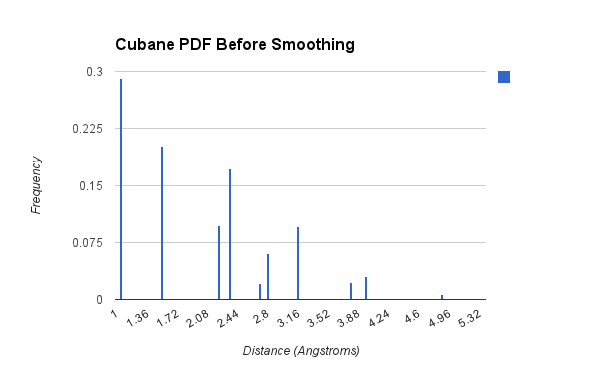
\includegraphics[scale=0.7]{figs/cubane_rdf_before_smoothing.png}
    \caption{Before Smoothing}
  \end{center}
\end{figure}

\begin{figure}
  \begin{center}
    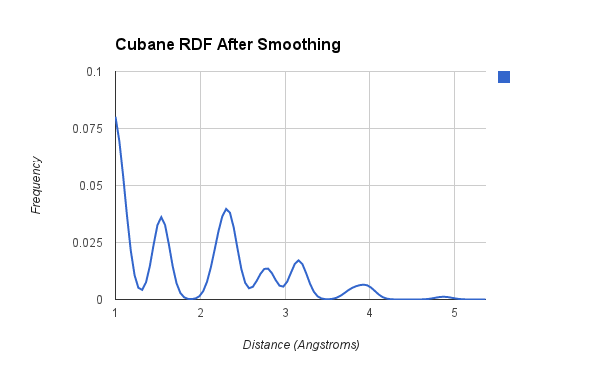
\includegraphics[scale=0.7]{figs/cubane_rdf_after_smoothing.png}
    \caption{After Smoothing}
  \end{center}
\end{figure}

\pagebreak

\noindent \textbf{Sources}
\begin{verbatim}
http://en.wikipedia.org/wiki/Atom_vibrations
http://en.wikipedia.org/wiki/Radial_distribution_function
\end{verbatim}

%\pagebreak
%\noindent \textbf{Appendix}\\
%\emph{Convolution Commutativity}\\
%\begin{align*}
%&\int_{- \infty}^\infty f(\tau) g(t - \tau) d\tau\\
%&u = t - \tau\\
%&\tau = -\infty \rightarrow u = \infty\\
%&\tau = \infty \rightarrow u = -\infty\\
%&du = -d\tau\\
%&- \int_\infty^{-\infty} f(t - u) g(u) du = \int_{-\infty}^\infty g(u) f(t-u)du\\
%\end{align*}

\end{document}
